\documentclass[letterpaper]{article}
\usepackage[margin=1in]{geometry}
\usepackage[utf8]{inputenc}
\usepackage{textcomp}
\usepackage{amssymb}
\usepackage{natbib}
\usepackage{graphicx}
\usepackage{gensymb}
\usepackage{amsthm, amsmath, mathtools}
\usepackage[dvipsnames]{xcolor}
\usepackage{enumerate}
\usepackage{mdframed}
\usepackage[most]{tcolorbox}
\usepackage{csquotes}
% https://tex.stackexchange.com/questions/13506/how-to-continue-the-framed-text-box-on-multiple-pages

\tcbuselibrary{theorems}

\newcommand{\R}{\mathbb{R}}
\newcommand{\Z}{\mathbb{Z}}
\newcommand{\N}{\mathbb{N}}
\newcommand{\Q}{\mathbb{Q}}
\newcommand{\C}{\mathbb{C}}
\newcommand{\code}[1]{\texttt{#1}}
\newcommand{\mdiamond}{$\diamondsuit$}
\newcommand{\PowerSet}{\mathcal{P}}
\newcommand{\Mod}[1]{\ (\mathrm{mod}\ #1)}
\DeclareMathOperator{\lcm}{lcm}

%\newtheorem*{theorem}{Theorem}
%\newtheorem*{definition}{Definition}
%\newtheorem*{corollary}{Corollary}
%\newtheorem*{lemma}{Lemma}
\newtheorem*{proposition}{Proposition}


\newtcbtheorem[number within=section]{theorem}{Theorem}
{colback=green!5,colframe=green!35!black,fonttitle=\bfseries}{th}

\newtcbtheorem[number within=section]{definition}{Definition}
{colback=blue!5,colframe=blue!35!black,fonttitle=\bfseries}{def}

\newtcbtheorem[number within=section]{corollary}{Corollary}
{colback=yellow!5,colframe=yellow!35!black,fonttitle=\bfseries}{cor}

\newtcbtheorem[number within=section]{lemma}{Lemma}
{colback=red!5,colframe=red!35!black,fonttitle=\bfseries}{lem}

\newtcbtheorem[number within=section]{example}{Example}
{colback=white!5,colframe=white!35!black,fonttitle=\bfseries}{def}

\newtcbtheorem[number within=section]{note}{Important Note}{
        enhanced,
        sharp corners,
        attach boxed title to top left={
            xshift=-1mm,
            yshift=-5mm,
            yshifttext=-1mm
        },
        top=1.5em,
        colback=white,
        colframe=black,
        fonttitle=\bfseries,
        boxed title style={
            sharp corners,
            size=small,
            colback=red!75!black,
            colframe=red!75!black,
        } 
    }{impnote}
\usepackage[utf8]{inputenc}
\usepackage[english]{babel}
\usepackage{fancyhdr}
\usepackage[hidelinks]{hyperref}

\pagestyle{fancy}
\fancyhf{}
\rhead{CSE 101}
\chead{Friday, February 18, 2022}
\lhead{Lecture 18}
\rfoot{\thepage}

\setlength{\parindent}{0pt}

\begin{document}

\section{Dynamic Programming}
Consider the Fibonacci sequence 
\[F_n = F_{n - 1} + F_{n - 2}\]
The naive algorithm would just recursively call $F_{n - 1}$ and $F_{n - 2}$, which is very inefficient, especially since we would be making duplicate calls. Instead, we can \emph{tabulate} the answers, thus saving us a bunch of time. 

\bigskip 

So, what is a dynamic program? The idea is as follows: 
\begin{enumerate}
    \item Relate your answer to some family of similar subproblems. In the case of Fibonacci, we had to relate the $n$th Fibonacci number to all of the Fibonacci numbers before it; that is, we had to compute $F_t$ for all $t \in [t, n] \subseteq \Z$.
    \item There should be a recurrence relation that gives the answer to each subproblem in terms of answers to simpler subproblems. 
    \item Create a \emph{table}, compute the answers to all subproblems, and then tabulate them (store the answers in the table so that you can refer back to the table when you need the answer from the previous iteration for your current iteration). This is done in the simplest to most complicated order. 
\end{enumerate}
\textbf{Remark:} You can \emph{usually} look up entries in the table in constant time. Generally speaking, the table is done using an array or a hash map. 

\bigskip 

A few notes about dynamic programming. 
\begin{itemize}
    \item The general correct proof outline is to prove by induction that each table entry is filled out correctly. Essentially, you want to make sure the base case is correct, and then make use of the recurrence relationship for the inductive hypothesis.
    \item The runtime of dynamic programming is \emph{usually} the number of subproblems \emph{multiplied by} the time per subproblem. 
    \item For finding the recurrence, which is very important in a dynamic programming algorithm, you often look at the first or last choice and see what things look like without that choice.
\end{itemize}


\subsection{Problem: Longest Common Subsequence}
Given a sequence $a_1 a_2 \dots a_n$, we can get a subsequence by removing some entries in the sequence. For example, if we have a sequence \code{ABCD}, a subsequence would be \code{ACD} (by removing the \code{B}). Given two sequences $a_1 a_2 \dots a_n$ and $b_1 b_2 \dots b_m$, then the common subsequence is just some $c_1 \dots c_k$ that is a subsequence of both $a_1 a_2 \dots a_n$ and $b_1 b_2 \dots b_m$. 

\bigskip 

So, the problem statement is as follows: Given two sequences, compute the longest common subsequences. That is, the subsequence with as many letters as possible. 

\subsubsection{Example: Longest Common Subsequence}
Suppose $X = \code{ABCBA}$ and $Y = \code{ABACA}$. Then, the longest common subsequence of $X$ and $Y$ is \code{ABCA}.

\subsubsection{Case Analysis}
How do we compute \code{LCSS}($A_1 A_2 \dots A_n$, $B_1 B_2 \dots B_m$)? We need to consider several cases for the common subsequence. 
\begin{enumerate}
    \item It does not use $A_n$ (it does not use the last letter in the sequence $A$). That is, if the common subsequence does not use $A_n$, it is actually a common subsequence of 
    \[A_1 A_2 A_{n - 1} \text{ and } B_1 B_2 \dots B_m\]
    Therefore, in this case, the longest common subsequence would be 
    \[\code{LCSS}(A_1 A_2 \dots A_{n - 1}, B_1 B_2 \dots B_m)\]


    \item It does not use $B_m$ (It does not use the last letter in the sequence $B$). If the common subsequence does not use $B_m$, it is actually a common subsequence of 
    \[A_1 A_2 A_n \text{ and } B_1 B_2 \dots B_{m - 1}\]
    Therefore, in this case, the longest common subsequence would be 
    \[\code{LCSS}(A_1 A_2 \dots A_n, B_1 B_2 \dots B_{m - 1})\]

    
    \item It uses both $A_n$ and $B_m$, and these characters are the same. If a common subsequence uses both $A_n$ and $B_m$, then:
    \begin{itemize}
        \item These characters must be the same.
        \item Such a subsequence can be obtained by taking a common subsequence of $A_1 A_2 \dots A_{n - 1}$ and $B_1 B_2 \dots B_{m - 1}$ and adding a copy of $A_n = B_m$ to the end. 
        \item Therefore, the longest length of such a subsequence is given by 
        \[\code{LCSS}(A_1 A_2 \dots A_n, B_1 B_2 \dots B_{m - 1}) + 1\]
    \end{itemize}
\end{enumerate}
\textbf{Remark:} We can be in both case 1 and case 2.

\subsubsection{Recursion}
We've broken the longest common subsequence into three different cases, and for each of these cases we managed to compute the longest common subsequence of subsequences in that case by a longest common subsequence problem that is a little bit simpler than the one that we started at. Of course, the \emph{best} longest common subsequence overall is just the best that we can get from any of these three cases. 

\bigskip 

So, all we need to do is look at the three cases and take the \emph{maximum} of the subsequences. That is
\[\code{LCSS}(A_1 A_2 \dots A_n, B_1 B_2 \dots B_m) = \max \begin{rcases}
    \begin{dcases}
        \code{LCSS}(A_1 A_2 \dots A_{n - 1}, B_1 B_2 \dots B_m) \\ 
        \code{LCSS}(A_1 A_2 \dots A_n, B_1 B_2 \dots B_{m - 1}) \\ 
        \code{LCSS}(A_1 A_2 \dots A_{n - 1}, B_1 B_2 \dots B_{m - 1})
    \end{dcases}
\end{rcases}\]
where the last option is allowed only if $A_n = B_m$. 

\subsubsection{Analyzing Recursive Calls}
Suppose we make a call to \code{LCSS}($A_1 \dots A_n$, $B_1 \dots B_m$). What recursive calls are made? 
\begin{center}
    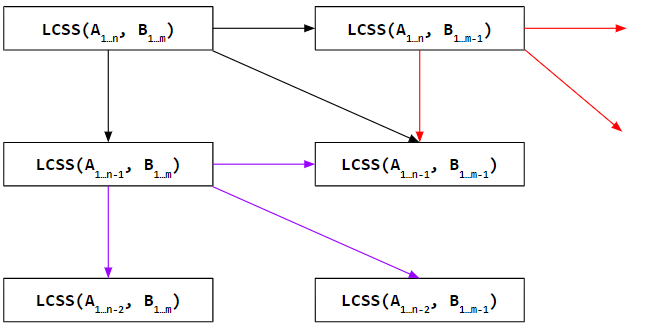
\includegraphics[scale=0.9]{../assets/lcss_1.png}
\end{center}
Here, many recursive calls are omitted. However, the key thing to note is that we're making a call to \code(LCSS)($A_1 A_2 \dots A_{n - 1}$, $B_1 B_2 \dots B_{m - 1}$) three times (there are three different paths to get to that function call). 

\begin{note}{}{}
    This is the key difference between a dynamic programming algorithm and a divide and conquer algorithm. 
    \begin{itemize}
        \item The recursive subcalls for a divide and conquer algorithm are significantly smaller than the original problem. So, you never have to compute that many recursive subcalls even if you do the entire recursion tree.
        \item The recursive subcalls for a dynamic program algorithm are almost as big as the original call. \emph{However}, the same subproblems will show up multiple times in the recursion tree. So, rather than recomputing each subproblem, we can compute each subproblem once and then \emph{store} the result so we can refer to it later if we need it. 
    \end{itemize}
    In the case of our problem above, we only ever see $\code{LCSS}(A_1 A_2 \dots A_k, B_1 B_2 \dots B_{\ell})$ for some $k$ and $\ell$. 
\end{note}

\subsubsection{Base Case}
Our recursion also needs a base case. So, our base case is: 
\[\code{LCSS}(\emptyset, B_1 B_2 \dots B_m) = \code{LCSS}(A_1 A_2 \dots A_n, \emptyset) = 0\]

\subsubsection{Algorithm}
To take advantage of the fact that our dynamic program makes multiple \emph{repeated} subcalls (i.e. subcalls with the same inputs), we use \emph{tabulation} to \emph{store} the results of one subcall and then, when needed, we can retrieve the results of the subcall. 

\bigskip 

Thus, our algorithm is\footnote{Because the \code{verbatim} environment is limiting, I'll represent $A_1 A_2 \dots A_n$ as $A[1..n]$ and $B_1 B_2 \dots B_m$ as $B[1..m]$.}: 
\begin{verbatim}
    LCSS(A[1..n], B[1..m]):
        Initialize Array T[0..n, 0..m]
        // T[i, j] will store LCSS(A[1..i, 1..j])
        For i = 0 to n: 
            For j = 0 to m:
                // Base Case 
                If i == 0 OR j == 0: 
                    T[i, j] = 0
                
                // Case (3)
                Else if A[i] == B[j]
                    T[i, j] = max(T[i - 1, j], T[i, j - 1], T[i - 1, j - 1] + 1)
                
                // Case (1) or (2)
                Else: 
                    T[i, j] = max(T[i - 1, j], T[i, j - 1])

        Return T[n, m]
\end{verbatim}
The runtime is as follows: 
\begin{itemize}
    \item The outer loop runs in $n$ time. 
    \item The inner loop runs in $m$ time. 
    \item Everything inside the inner loop runs in constant time. 
\end{itemize}
This gives us the runtime $\BigO(nm)$. 

\subsubsection{Example: Longest Common Subsequence Redux}
Suppose $X = \code{ABCBA}$ and $Y = \code{ABACA}$. Find the longest common subsequence.

\begin{mdframed}[]
    We will tabulate the process. Call the table $T$. 
    \begin{center}
        \begin{tabular}{|c|c|c|c|c|c|c|}
            \hline 
                & $\emptyset$ & \code{A} & \code{AB} & \code{ABA} & \code{ABAC} & \code{ABACA} \\
            \hline 
            $\emptyset$     &   &   &   &   &   & \\ 
            \hline
            \code{A}        &   &   &   &   &   & \\ 
            \hline
            \code{AB}       &   &   &   &   &   & \\ 
            \hline
            \code{ABC}      &   &   &   &   &   & \\ 
            \hline
            \code{ABCB}     &   &   &   &   &   & \\ 
            \hline
            \code{ABCBA}    &   &   &   &   &   & \\ 
            \hline
        \end{tabular}
    \end{center}

    We will go through each table one row at a time. 
    \begin{enumerate}
        \item If we start at \code{i = 0}, then regardless of the value of \code{j}, the entire first row will be \code{0} by the first \code{if}-condition. So: 
        \begin{center}
            \begin{tabular}{|c|c|c|c|c|c|c|}
                \hline 
                    & $\emptyset$ & \code{A} & \code{AB} & \code{ABA} & \code{ABAC} & \code{ABACA} \\
                \hline 
                $\emptyset$     & 0 & 0 & 0 & 0 & 0 & 0 \\ 
                \hline
                \code{A}        &   &   &   &   &   &   \\ 
                \hline
                \code{AB}       &   &   &   &   &   &   \\ 
                \hline
                \code{ABC}      &   &   &   &   &   &   \\ 
                \hline
                \code{ABCB}     &   &   &   &   &   &   \\ 
                \hline
                \code{ABCBA}    &   &   &   &   &   &   \\ 
                \hline
            \end{tabular}
        \end{center}

        \item Now, when \code{i = 1}, then we need to consider the value of \code{j}. 
        \begin{itemize}
            \item If \code{j = 0}, then the entry at \code{T[1, 0] = 0}.
            
            \item If \code{j = 1}, then we're comparing \code{A} with \code{A}, so we need to consider the second \code{if}-condition. In this case, we need to check the entry directly above (\code{T[i - 1, j]}), to the left (\code{T[i, j - 1]}), and directly adjacent in the top-left entry (\code{T[i - 1, j - 1] + 1}). Here, we see that the values are \code{0}, \code{0}, and \code{0 + 1 = 1}, respectively. So, we store the \emph{maximum} of these values in \code{T[1, 1]}. Thus, \code{T[1, 1] = 1}. 
            
            \item If \code{j = 2}, then we're comparing \code{A} with \code{AB}, so we need to consider the third \code{if}-condition. In this case, we check the entry directly above \code{T[i - 1, j]} and directly to the left (\code{T[i, j - 1]}), and take the maximum. In our case, we have \code{0} and \code{1} (which we computed from the previous bullet point), respectively. Thus, \code{T[1, 2] = 1}.
            
            \item If \code{j = 3}, then we're comparing \code{A} with \code{AB}, so we need to consider the second \code{if}-condition. In this case, we check the entry directly above, left, and adjacent (add one to the end result) of \code{[i, j] = [1, 3]}. We get the values \code{0}, \code{1}, and \code{0 + 1 = 1}, respectively. Thus, \code{T[1, 3] = 1}.  
            
            \item Continuing on, we get \code{1}'s for the remaining cells in this row. 
        \end{itemize}
        Therefore, the second row is: 
        \begin{center}
            \begin{tabular}{|c|c|c|c|c|c|c|}
                \hline 
                    & $\emptyset$ & \code{A} & \code{AB} & \code{ABA} & \code{ABAC} & \code{ABACA} \\
                \hline 
                $\emptyset$     & 0 & 0 & 0 & 0 & 0 & 0 \\ 
                \hline
                \code{A}        & 0 & 1 & 1 & 1 & 1 & 1 \\ 
                \hline
                \code{AB}       &   &   &   &   &   &   \\ 
                \hline
                \code{ABC}      &   &   &   &   &   &   \\ 
                \hline
                \code{ABCB}     &   &   &   &   &   &   \\ 
                \hline
                \code{ABCBA}    &   &   &   &   &   &   \\ 
                \hline
            \end{tabular}
        \end{center}

        Omitting the rest of the work, we see that the result is: 
        \begin{center}
            \begin{tabular}{|c|c|c|c|c|c|c|}
                \hline 
                    & $\emptyset$ & \code{A} & \code{AB} & \code{ABA} & \code{ABAC} & \code{ABACA} \\
                \hline 
                $\emptyset$     & 0 & 0 & 0 & 0 & 0 & 0 \\ 
                \hline
                \code{A}        & 0 & 1 & 1 & 1 & 1 & 1 \\ 
                \hline
                \code{AB}       & 0 & 1 & 2 & 2 & 2 & 2 \\ 
                \hline
                \code{ABC}      & 0 & 1 & 2 & 2 & 3 & 3 \\ 
                \hline
                \code{ABCB}     & 0 & 1 & 2 & 2 & 3 & 3 \\ 
                \hline
                \code{ABCBA}    & 0 & 1 & 2 & 3 & 3 & 4 \\ 
                \hline
            \end{tabular}
        \end{center}
        And so the answer is given by the bottom-right entry, or \boxed{\code{4}}. 
    \end{enumerate}
\end{mdframed}

\subsubsection{Finding the Longest Common Subsequence}
The above algorithm finds the \emph{length} of the longest common subsequence. What if we wanted the actual subsequence? Well, we can \emph{backtrack}. So, consider the table above. 
\begin{center}
    \begin{tabular}{|c|c|c|c|c|c|c|}
        \hline 
            & $\emptyset$ & \code{A} & \code{AB} & \code{ABA} & \code{ABAC} & \code{ABACA} \\
        \hline 
        $\emptyset$     & 0 & 0 & 0 & 0 & 0 & 0 \\ 
        \hline
        \code{A}        & 0 & 1 & 1 & 1 & 1 & 1 \\ 
        \hline
        \code{AB}       & 0 & 1 & 2 & 2 & 2 & 2 \\ 
        \hline
        \code{ABC}      & 0 & 1 & 2 & 2 & 3 & 3 \\ 
        \hline
        \code{ABCB}     & 0 & 1 & 2 & 2 & 3 & 3 \\ 
        \hline
        \code{ABCBA}    & 0 & 1 & 2 & 3 & 3 & 4 \\ 
        \hline
    \end{tabular}
\end{center}
We can use this trick, based on the recurrence, to find out what the subsequence is. If you're at \code{[i, j]}, consider the neighbors \code{[i - 1, j]}, \code{[i, j - 1]}, and \code{[i - 1, j - 1]}. 
\begin{itemize}
    \item If the values at all three of those entries are equal, then take the diagonal path; that is, take \code{[i - 1, j - 1]}.
    \item If \code{[i - 1, j - 1]} and \code{[i - 1, j]} are equal but \code{[i, j - 1]} isn't equal to any of those two, then take the \code{[i, j - 1]} path. 
    \item If \code{[i - 1, j - 1]} and \code{[i, j - 1]} are equal but \code{[i - 1, j]} isn't equal to any of those two, then take the \code{[i - 1, j]} path. 
\end{itemize}
Once you reach the beginning, then you backtrack again. For each \emph{diagonal} path that was taken, take the last letter of one of the subsequences (the subsequences corresponding to the cell should end with the same letter). Once you reach back to the bottom-right square, then you can just concatenate the letters that you found.
\begin{center}
    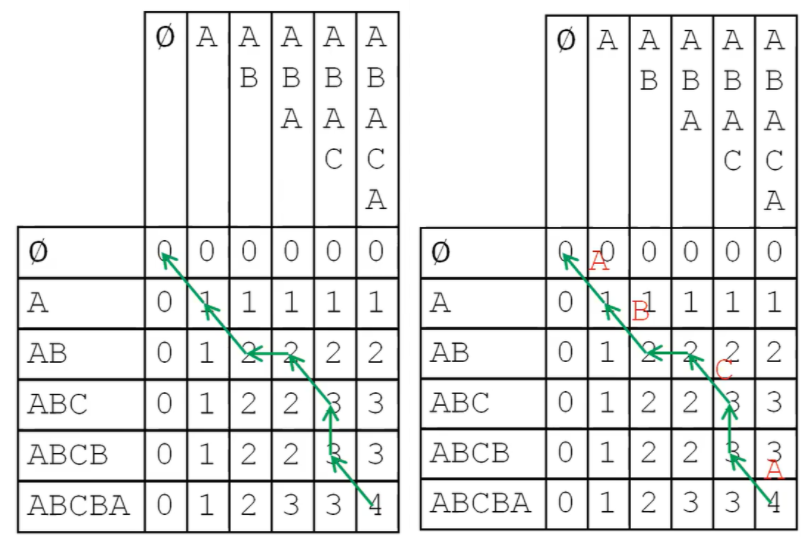
\includegraphics[scale=0.7]{../assets/lcss_2.png}
\end{center}


\subsubsection{Proof of Correctness}
We now need to prove, by induction, that this algorithm is correct. 

\begin{mdframed}[]
    \begin{proof}
        We will use induction on $i$, $j$ to show that the value assigned to $T[i, j]$ is the correct value for \code{LCSS}($A_1 \dots A_i$, $B_1 \dots B_j$).
        \begin{itemize}
            \item \underline{Base Case:} When $i = 0 $ or $j = 0$, then we assign \code{0} since the empty string has no common subsequence with a string of some length. 
            \item \underline{Inductive Step:} Suppose the previous values are assigned correctly. We note that, because of the recursive relationship and the inductive hypothesis (since we have previously filled out $T[i - 1, j]$, $T[i, j - 1]$, and $T[i - 1, j - 1]$ correctly), that $T[i, j]$ gets the correct values. 
        \end{itemize}
        This completes the proof. 
    \end{proof}
\end{mdframed}

\end{document}